%%%%%%%%%%%%%%%%%%%%%%%%%%%%%%%%%%%%%%%%%%%%%%%%%%%%%%%%%%%%%%%%%%%%%%
% Overleaf (WriteLaTeX) Example: Molecular Chemistry Presentation
%
% Source: http://www.overleaf.com
%
% In these slides we show how Overleaf can be used with standard 
% chemistry packages to easily create professional presentations.
% 
% Feel free to distribute this example, but please keep the referral
% to overleaf.com
% 
%%%%%%%%%%%%%%%%%%%%%%%%%%%%%%%%%%%%%%%%%%%%%%%%%%%%%%%%%%%%%%%%%%%%%%

\documentclass{beamer}

\mode<presentation>
{
  \usetheme{Madrid}       % or try default, Darmstadt, Warsaw, ...
  \usecolortheme{default} % or try albatross, beaver, crane, ...
  \usefonttheme{default}    % or try default, structurebold, ...
  \setbeamertemplate{navigation symbols}{}
  \setbeamertemplate{caption}[numbered]
} 

\usepackage[english]{babel}
\usepackage[utf8x]{inputenc}
\usepackage{chemfig}
\usepackage[version=3]{mhchem}

\usepackage{hyperref}
  \hypersetup{colorlinks=true}
  \hypersetup{urlcolor=blue}
  \hypersetup{linkcolor = .}
\usepackage{xcolor}
\usepackage{siunitx}
  \sisetup{separate-uncertainty = true}
\usepackage{physics}
\usepackage[font=small,labelfont=bf]{caption}
\usepackage{subcaption}
\usepackage[en-GB]{datetime2}
\usepackage{overpic}
\usepackage{feynmp}
\DeclareGraphicsRule{*}{mps}{*}{}

\usepackage{scalerel}
\newcommand{\mylbrace}[2]{\vspace{#2pt}\hspace{6pt}\scaleleftright[\dimexpr5pt+#1\dimexpr0.06pt]{\lbrace}{\rule[\dimexpr2pt-#1\dimexpr0.5pt]{-4pt}{#1pt}}{.}}
\newcommand{\myrbrace}[2]{\vspace{#2pt}\scaleleftright[\dimexpr5pt+#1\dimexpr0.06pt]{.}{\rule[\dimexpr2pt-#1\dimexpr0.5pt]{-4pt}{#1pt}}{\rbrace}\hspace{6pt}}

% Here's where the presentation starts, with the info for the title slide
\title[University of Oxford]{BESIII Charm Meeting \\Measurement of $\delta_D^{K\pi}$ with $D\to K_{S, L}\pi^+\pi^-$ tags}
\author{Martin Tat}
\institute{University of Oxford}
\date{31st August 2021}

\titlegraphic{
\includegraphics[width = 2.5cm, height = 2.5cm]{OxfordLogo.pdf}\hspace{1cm}~%
              
\includegraphics[width = 3.5cm, height = 2.5cm]{bes3.jpg}}

\begin{document}

\begin{frame}
  \titlepage
\end{frame}

% These three lines create an automatically generated table of contents.
%\begin{frame}{Outline}
%  \tableofcontents
%\end{frame}

\begin{frame}{$D\to K_{S, L}^0\pi^+\pi^-$ tags}
  \begin{center}
    {\huge Measurement of $\delta_D^{K\pi}$ with $D\to K_{S, L}\pi^+\pi^-$ tags}
  \end{center}
  \begin{columns}
    \column{0.50\linewidth}
    \begin{itemize}
      \setlength\itemsep{1.0em}
      \item{Measurement of \underline{both} $r_D^{K\pi}\cos\delta_D^{K\pi}$ and $r_D^{K\pi}\sin\delta_D^{K\pi}$}
      \item{Equal-$\Delta\delta_D$ phase space binning}
      \item{Double tag yields taken from \href{https://doi.org/10.1103/PhysRevD.101.112002}{Phys. Rev. D \textbf{101} (2020)}}
      \item{$K_i$, $c_i$, $s_i$ re-determined without $D\to K^-\pi^+$ inputs (by Lei Li)}
    \end{itemize}
    \column{0.50\linewidth}
    \centering
    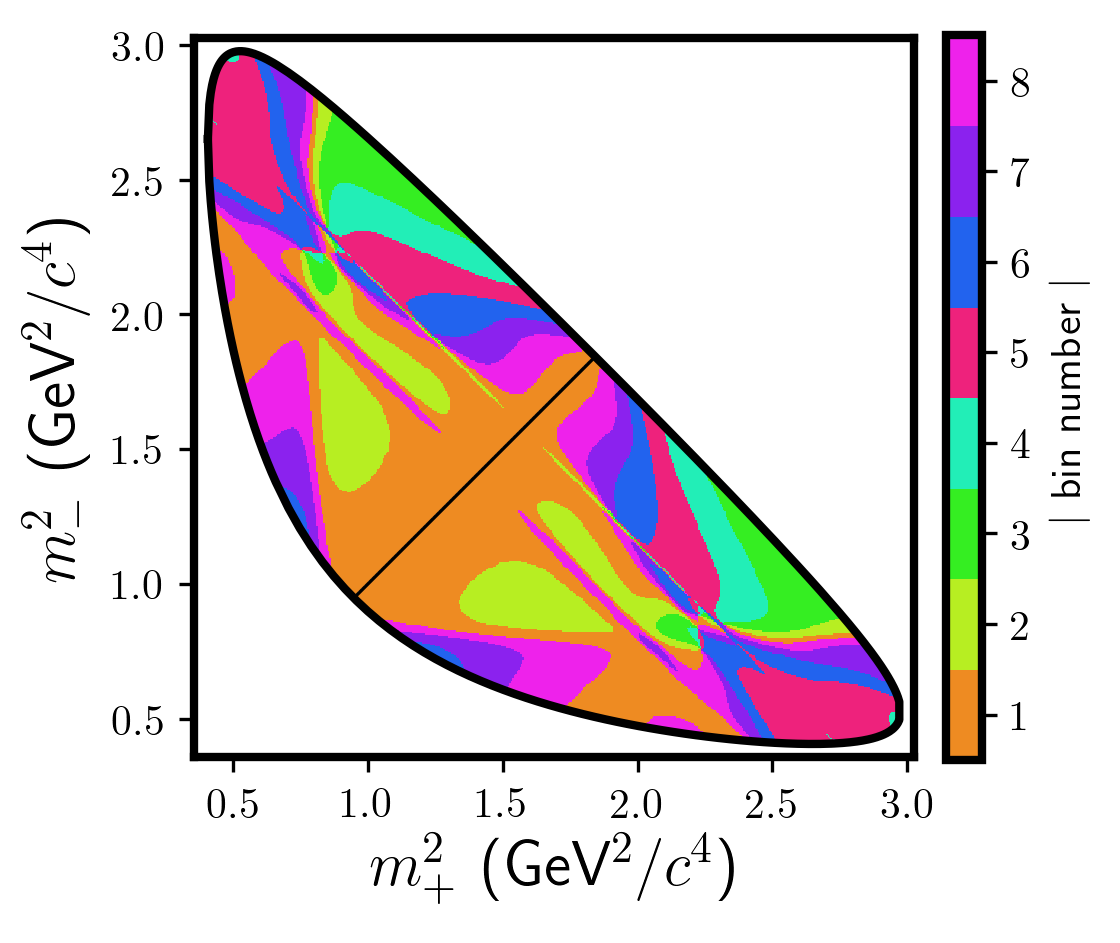
\includegraphics[width=\textwidth]{KsPiPi_equal.png}
  \end{columns}
\end{frame}

\begin{frame}{$D\to K_{S, L}^0\pi^+\pi^-$ inputs}
  \begin{block}{$K^-\pi^+$ vs $K_{S, L}^0\pi^+\pi^-$ double tag yield prediction}
    $Y(K^-\pi^+|K_{S, L}^0\pi^+\pi^-)_i =$ \\ 
    $H^{(\prime)}\Big(K_i^{(\prime)} + \big(r_D^{K\pi}\big)^2K_{-i}^{(\prime)} \mp 2r_D^{K\pi}\sqrt{K_i^{(\prime)}K_{-i}^{(\prime)}}\big[c_i^{(\prime)}\cos\delta_D^{K\pi} - s_i^{(\prime)}\sin\delta_D^{K\pi}\big]\Big)$
  \end{block}
  \begin{itemize}
      \setlength\itemsep{1.0em}
    \item{$K_i$: Flavour tag yields}
    \begin{itemize}
      \setlength\itemsep{0.5em}
      \item{$D\to K_{S, L}^0\pi^+\pi^-$ vs $D\to K^-\pi^+\pi^0$}
      \item{$D\to K_{S, L}^0\pi^+\pi^-$ vs $D\to K^-\pi^+\pi^-\pi^+$}
      \item{$D\to K_S^0\pi^+\pi^-$ vs $D\to K^-e^+\nu_e$}
      \item{Updated coherence factors from \href{https://doi.org/10.1007/JHEP05(2021)164}{J. High Energ. Phys. \textbf{2021}, 164}}
    \end{itemize}
    \item{$c_i$ and $s_i$: Amplitude-averaged strong phases}
    \begin{itemize}
      \setlength\itemsep{0.5em}
      \item{Updated with no $D\to K^-\pi^+$ inputs}
    \end{itemize}
  \end{itemize}
\end{frame}

\begin{frame}{Fit setup and results}
  \begin{itemize}
    \setlength\itemsep{1.0em}
    \item{Minimize $\chi^2 = \sum\Big(\frac{Y_{\rm obs} - Y_{\rm exp}}{\Delta Y_{\rm obs}}\Big)^2$}
    \begin{itemize}
      \item{$\Delta Y_{\rm obs}$ statistical uncertainty only}
    \end{itemize}
    \item{Systematic uncertainties: Run $10^5$ fits with smearing}
    \begin{itemize}
      \item{$K_i$: Independent Gaussian smearing according to uncertainties}
      \item{$c_i$, $s_i$: Gaussian smearing according to correlations and uncertainties}
    \end{itemize}
  \end{itemize}
  \begin{block}{Final results}
    \vspace{0.1cm}
    $r_D^{K\pi}\cos\delta_D^{K\pi} = -0.0547\pm0.0084\pm0.0049\pm0.0010$ \\
    \vspace{0.3cm}
    $r_D^{K\pi}\sin\delta_D^{K\pi} = -0.010\pm0.012\pm0.007\pm0.003$ \\
    \vspace{0.1cm}
    Uncertainties: Statistical $\pm$ $K_i$ systematics $\pm$ $c_i$/$s_i$ systematics
  \end{block}
  \vspace{-0.2cm}
  \begin{columns}
    \column{0.50\linewidth}
    \begin{itemize}
      \vspace{0.1cm}
      \item{$r_D^{K\pi}\cos\delta_D^{K\pi}$/$r_D^{K\pi}\sin\delta_D^{K\pi}$ correlations are small:}
    \end{itemize}
    \column{0.50\linewidth}
    \begin{tabular}{lrrr}
      \\
      \hline
      $K^-\pi^+$ & $K_i^{(\prime)}$ & $c_i^{(\prime)}, s_i^{(\prime)}$ \\
      \hline
      0.035      & -0.005           & 0.021 \\
      \hline
    \end{tabular}
  \end{columns}
\end{frame}

\begin{frame}{Bin yield yield vs fit prediction}
  \begin{figure}
    \centering
    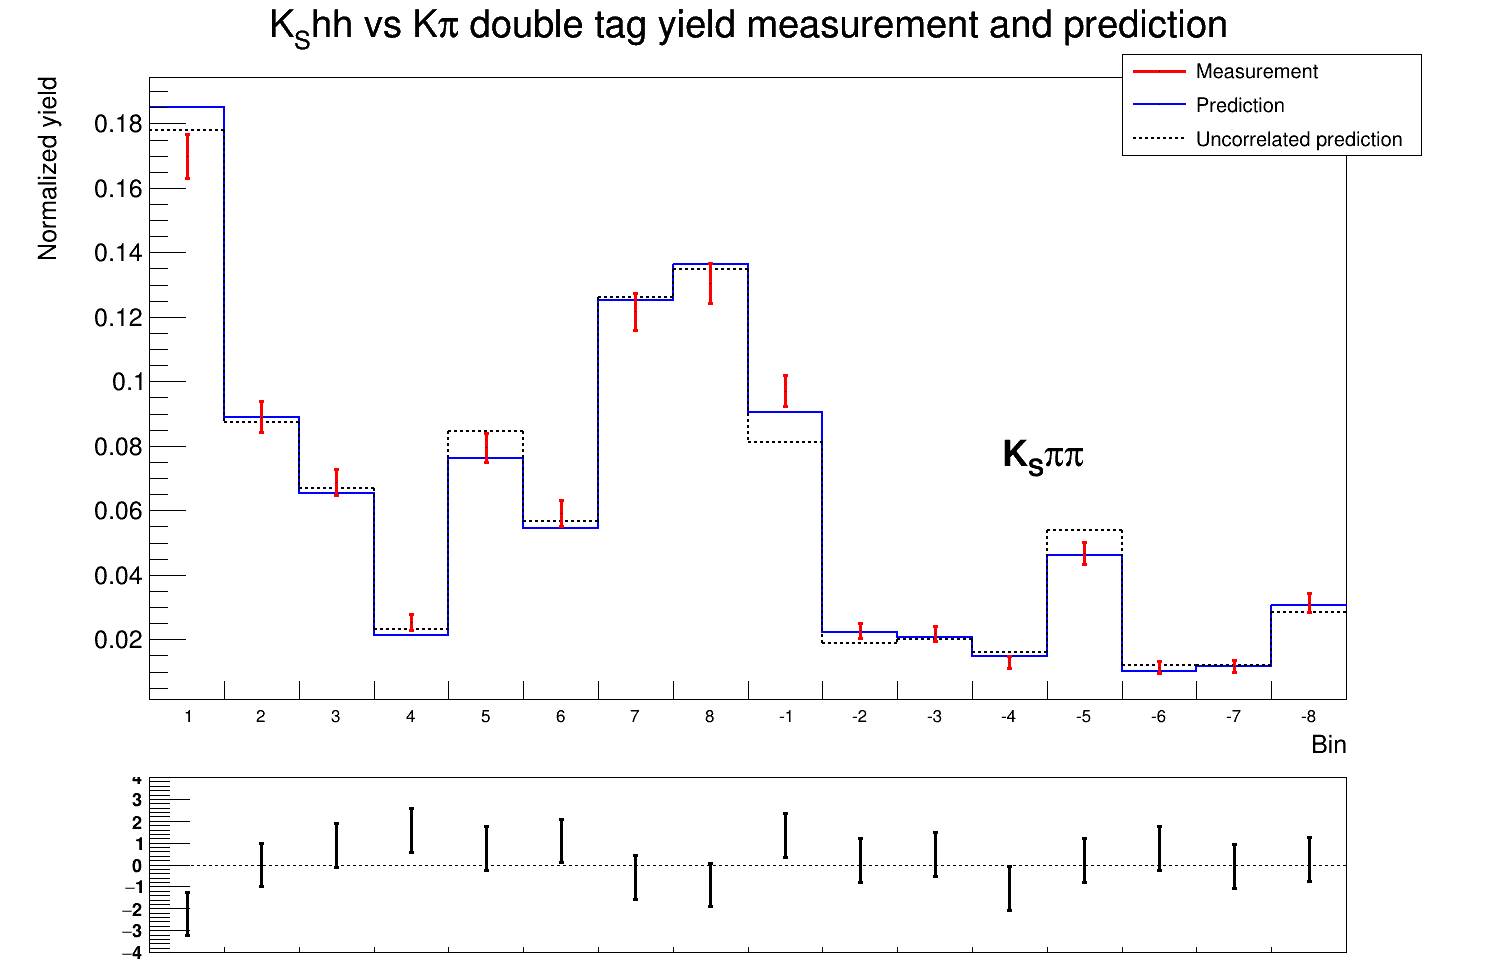
\includegraphics[width=\textwidth]{KSpipiVersusKpiYields.png}
  \end{figure}
\end{frame}

\begin{frame}{Bin yield yield vs fit prediction}
  \begin{figure}
    \centering
    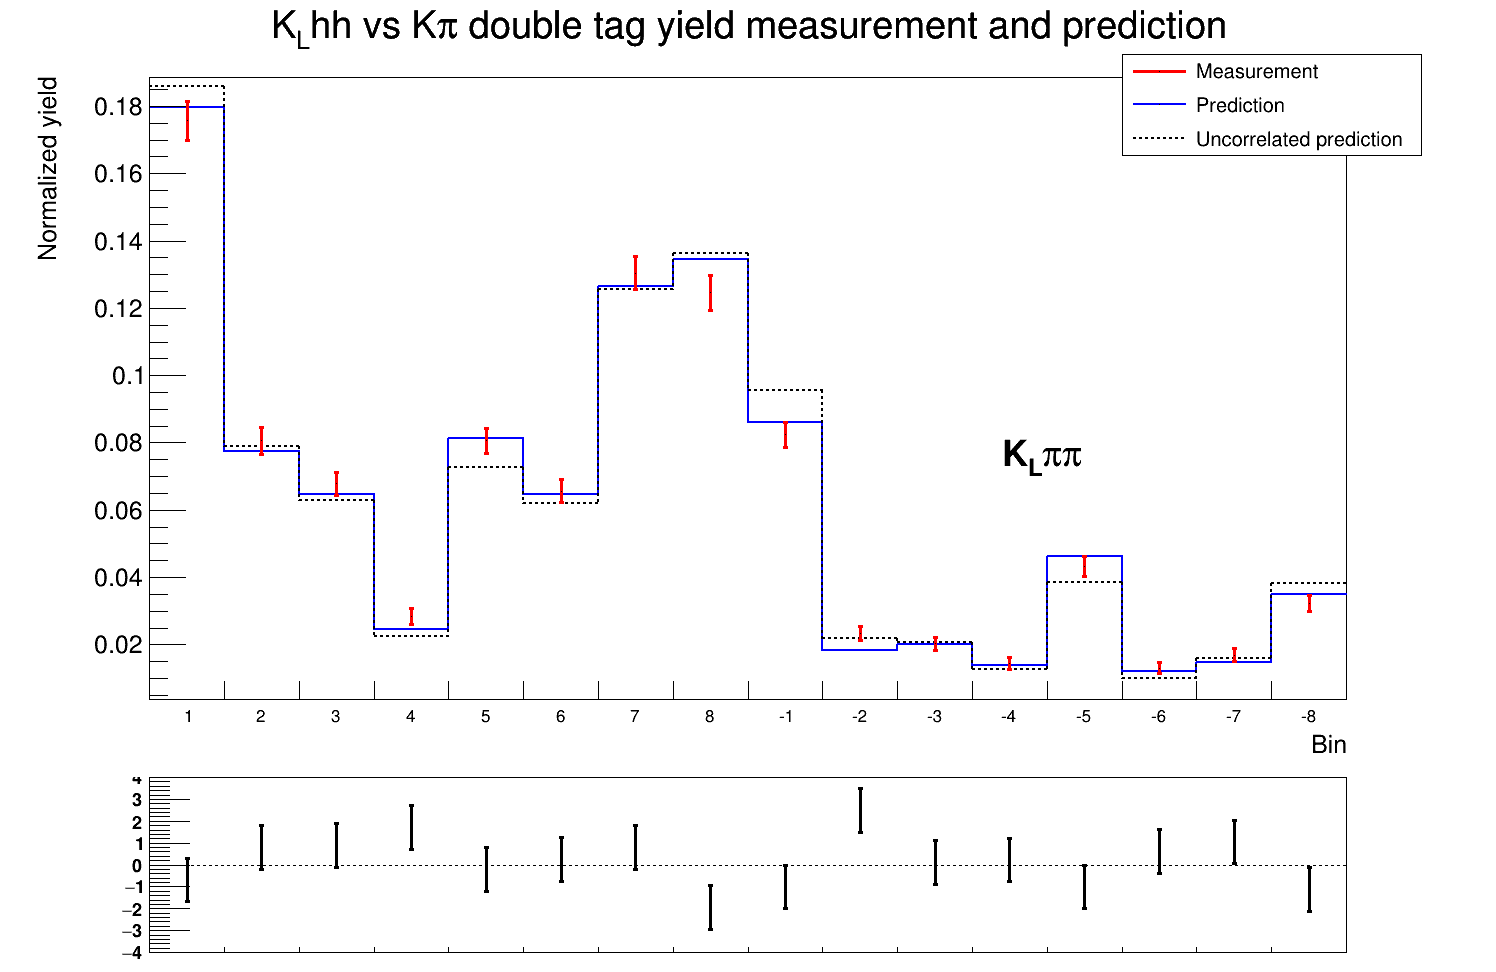
\includegraphics[width=\textwidth]{KLpipiVersusKpiYields.png}
  \end{figure}
\end{frame}

\begin{frame}{Separate $K_S^0\pi^+\pi^-$ and $K_L^0\pi^+\pi^-$ fits}
  \begin{figure}
    \centering
    \begin{subfigure}{0.5\textwidth}
      \centering
      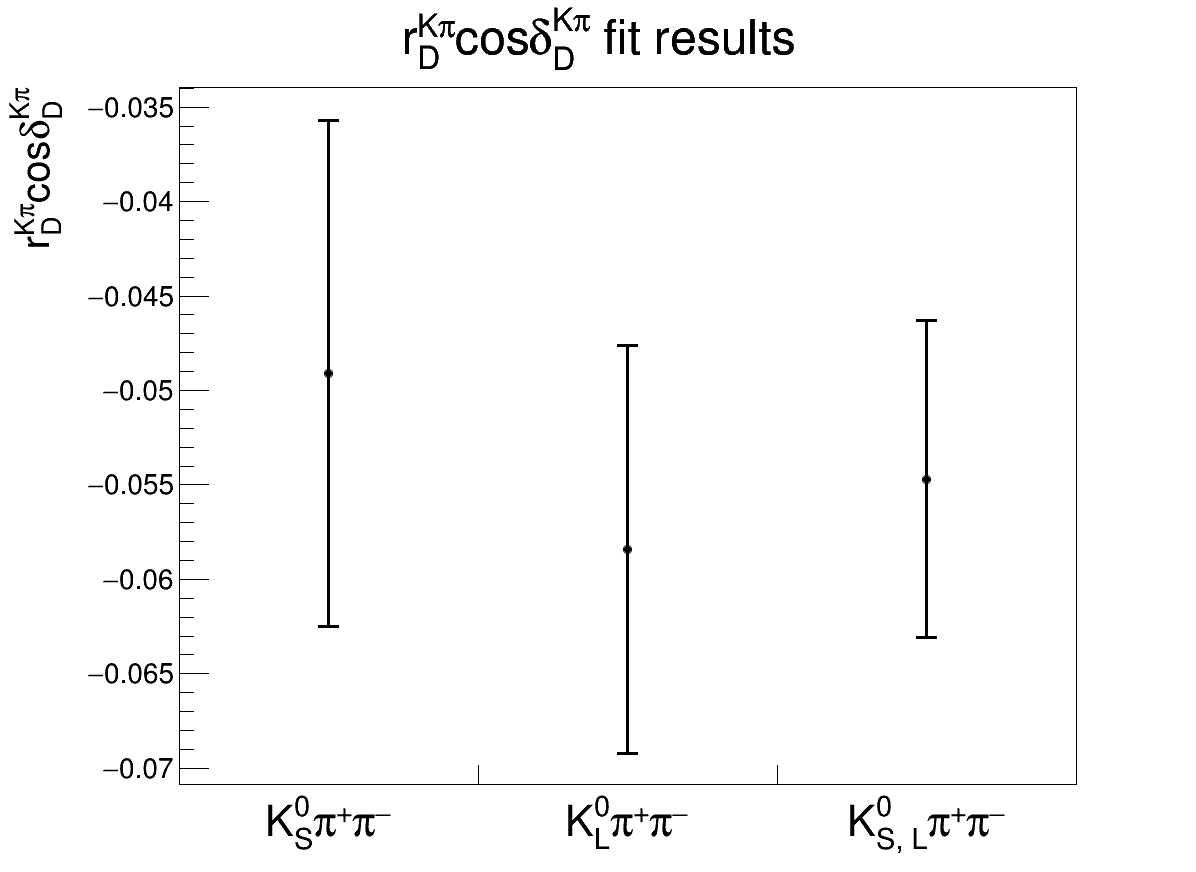
\includegraphics[width=\textwidth]{rDcosDeltaK0pipi.png}
    \end{subfigure}%
    \begin{subfigure}{0.5\textwidth}
      \centering
      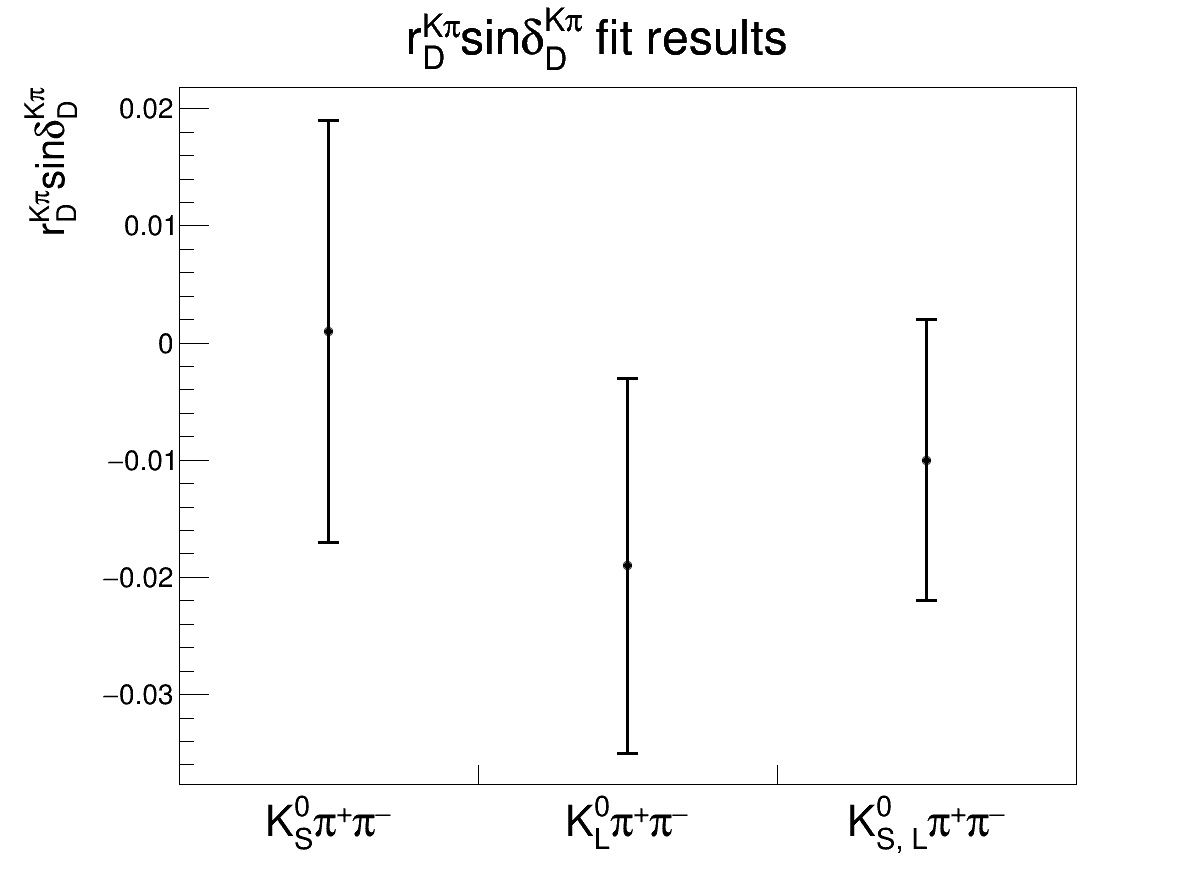
\includegraphics[width=\textwidth]{rDsinDeltaK0pipi.png}
    \end{subfigure}
  \end{figure}
  \centering
  \begin{tabular}{lrrr}
    \hline
    Sample                 & $r_D^{K\pi}\cos\delta_D^{K\pi}$ & $r_D^{K\pi}\sin\delta_D^{K\pi}$ & $\chi^2/{ndf}$ \\
    \hline
    $K^0_S \pi^+\pi^-$     & -0.0491 $\pm$ 0.0134 &  0.001 $\pm$ 0.018 & 14.4/14 \\
    $K^0_L \pi^+\pi^-$     & -0.0584 $\pm$ 0.0108 & -0.019 $\pm$ 0.016 & 20.1/14 \\
    $K^0_{S,L} \pi^+\pi^-$ & -0.0547 $\pm$ 0.0084 & -0.010 $\pm$ 0.012 & 35.4/30 \\
    CP tags                & -0.0605 $\pm$ 0.0053 & - & \\
    \hline
  \end{tabular}
\end{frame}

\begin{frame}{Combination of measurements}
  \begin{columns}
    \column{0.35\linewidth}
    Inputs to combination:
    \vspace{0.3cm}
    \begin{itemize}
      \setlength\itemsep{2.0em}
      \item{$r_D^{K\pi}\cos\delta_D^{K\pi} = \SI{-0.0588(52)}{}$}
      \begin{itemize}
        \item{$K_{S, L}^0\pi^+\pi^-$}
        \item{CP tags}
      \end{itemize}
      \item{$r_D^{K\pi}\sin\delta_D^{K\pi} = \SI{-0.010(14)}{}$}
      \begin{itemize}
        \item{$K_{S, L}^0\pi^+\pi^-$}
      \end{itemize}
    \end{itemize}
    Final result:
    \vspace{0.3cm}
    \begin{itemize}
      \setlength\itemsep{0.5em}
      \item{$\delta_D^{K\pi} = \big(188.7^{+11.2}_{-13.0}\big)^\circ$}
      \item{$\delta_D^{K\pi} = \big(189.8^{+14.3}_{-13.7}\big)^\circ$ from $r_D^{K\pi}\sin\delta_D^{K\pi}$ only}
    \end{itemize}
    \column{0.65\linewidth}
    \begin{figure}
      \centering
      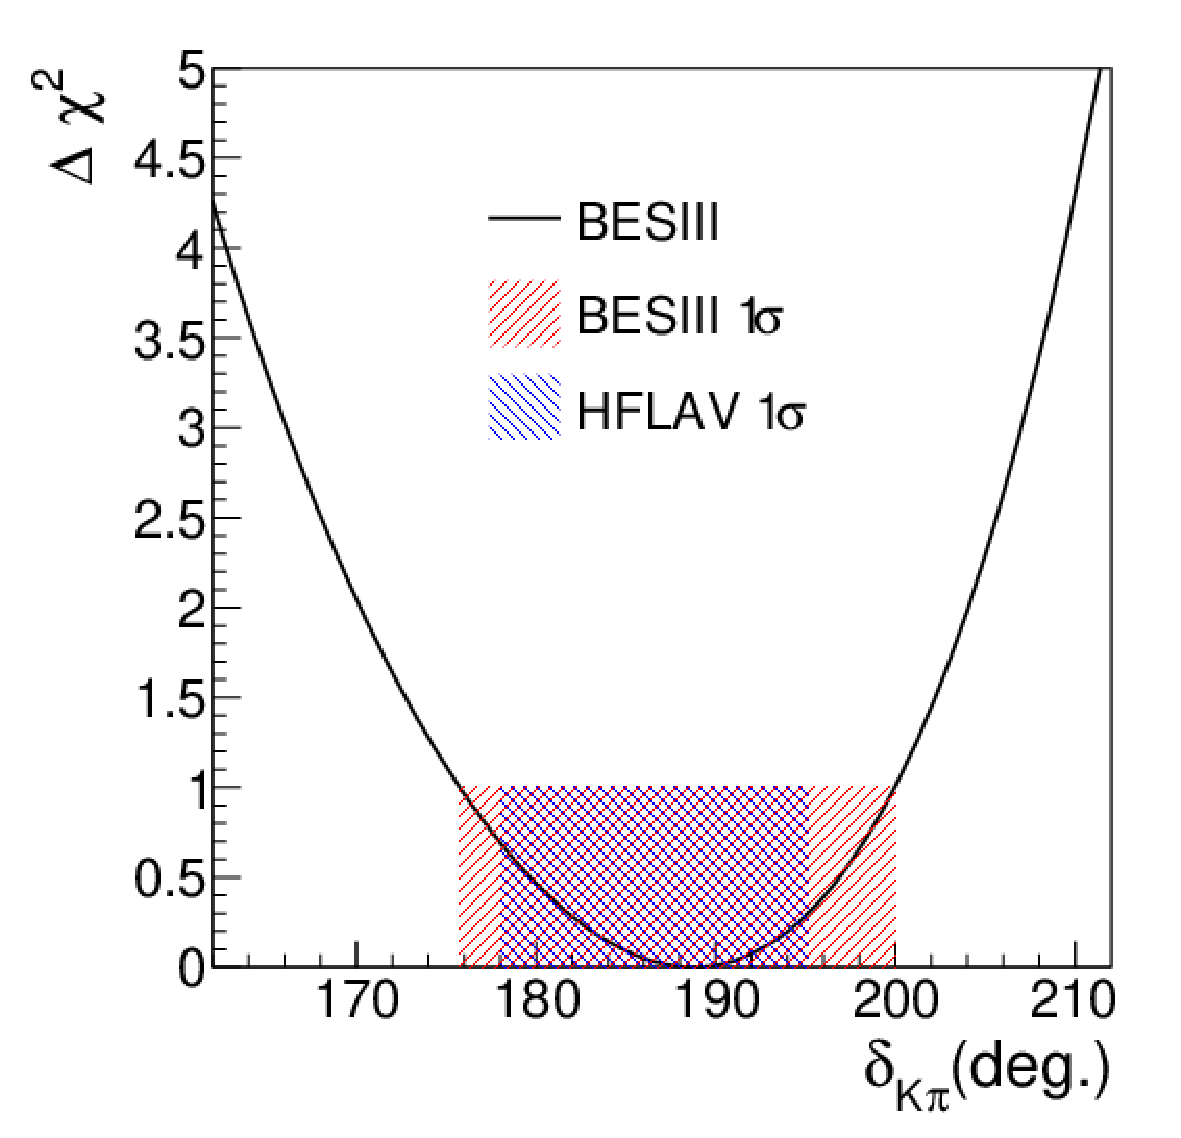
\includegraphics[width=\textwidth]{delta_kpi_combination.pdf}
    \end{figure}
  \end{columns}
\end{frame}

\begin{frame}{Summary}
  \begin{itemize}
    \item{Have performed an updated measurement of $\mathcal{A}_{K\pi} = \SI{0.127(12)}{}$}
    \item{As part of this analysis, BR of three $K_LX$ modes in a manner independent of flavour-tag input were determined}
    \begin{itemize}
      \item{These will be valuable inputs for future strong-phase studies}
    \end{itemize}
    \item{Have fitted $K^-\pi^+$ vs $K_{S, L}\pi^+\pi^-$ in bins of phase space}
    \begin{itemize}
      \item{Gain sensitivity to both $r_D^{K\pi}\cos\delta_D^{K\pi}$ and $r_D^{K\pi}\sin\delta_D^{K\pi}$}
    \end{itemize}
    \item{Final result: $\delta_D^{K\pi} = \big(188.7^{+11.2}_{-13.0}\big)^\circ$}
    \item{Precision compares favourably with that from ensemble of charm-mixing data, will improve significantly with increase in data set foreseen at $\psi(3770)$}
    \item{MEMO in preparation, and will be circulated in coming week}
  \end{itemize}
  \begin{center}
    {\huge Thank you!}
  \end{center}
\end{frame}
    

\end{document}
